\chapter{App. Methods: Quasi-classical approximation}
Material for this chapter can be found in the books by Migdal and Bender and Orszag.\par
The quasi-classical or WKB (Wentzel-Kramers-Brillouin) method has a physical, a mathematical, and a practical aspect. We start with the physical aspect and make the following approach for the wave function $\Psi(\vec{r},t)$, where $A(\vec{r},t)$ and $S(\vec{r},t)$ are real-valued functions,
%公式 1
\begin{equation}
    \Psi(\vec{r}, t)=A(\vec{r}, t) \exp \left[\frac{i}{\hbar} S(\vec{r}, t)\right]
\end{equation}

Inserting it into the Schrodering equation with $H = p^2 / 2m + V (\vec{r})$ and separation into real and imaginary parts results
%公式 2

\begin{align} \partial_{t} S+\frac{(\vec{\nabla} S)^{2}}{2 m}+V &=\frac{\hbar^{2}}{2 m} \frac{\Delta A}{A} \\ m \partial_{t} A+(\vec{\nabla} A \cdot \vec{\nabla} S)+\frac{A}{2} \Delta S &=0 \end{align}

%公式 3
With the definition (10.1) we get the probability density $\rho=A^2$ and the current density $\vec{j}=A^2\vec{\nabla}S/m$. The formula (10.3) leads to the continuity equation: the multiplication by $2A / m$ results

%公式 4
\begin{equation}
    \partial_{t} A^{2}+\vec{\nabla}\left(A^{2} \vec{\nabla} S / m\right)=0
    \end{equation}
Note that (10.3) does not depend on $\hbar$ and is therefore already a classic equation. The classic limit - i.e. $\hbar\rightarrow 0$- of (10.2) is
%公式 5
\begin{equation}
    \partial_{t} S+\frac{(\vec{\nabla} S)^{2}}{2 m}+V=0
    \end{equation}
This can also be written as
%公式 6
\begin{equation}
    H\left(p_{i}=\partial S / \partial x_{i}, x_{j}\right)+\partial_{t} S=0
    \end{equation}
which is the Hamilton-Jacobi equation for the corresponding classical problem. 1
We define the velocity $\vec{v}=\vec{j}/\rho=\vec{\nabla}S/m$  and find the hydrodynamic problem with (10.4) and (10.5)\footnote{The partial differential equation (10.6) is solved by $S (x_j, \alpha_i; t) + S_0$ with the integration constants $\alpha_i$ and $S_0$. Substitution of the integration constant αi by pulses $P_i$ gives the generator $S (x_j, P_i; t)$. $S$ generates the trivial problem via the canonical transformation $p_{\nu}=\partial S/\partial x_{\nu},X_{\mu}=\partial S/\partial P_{\mu}$
\begin{equation}
    \widetilde{H}\left(P_{i}, X_{j}\right)=0 ; \quad-\dot{P}_{\nu}=\frac{\partial \widetilde{H}}{\partial X_{\nu}}=0, \quad \dot{X}_{\mu}=\frac{\partial \widetilde{H}}{\partial P_{\mu}}=0
    \end{equation}
with solutions $P_{\nu}$ = const = $\alpha_{\nu}$ and $X_{\mu}$ = const. = $\beta_{\mu}$. The canonical transformation $X_{\mu},P_{\nu}\leftrightarrow x_j,p_i$ gives the mechanical path in the original coordinates ¨ $x_j$. Inserting in $S$ gives the effect
\begin{equation}
    S(t)=S\left(x_{j}(t), \alpha_{i} ; t\right)=\int_{t_{0}}^{t} L\left(t^{\prime}\right) d t^{\prime}+S\left(t_{0}\right)
    \end{equation}
    along the train. This gives us the approximation
    \begin{equation}
        \Psi \sim e^{iS/\hbar}
    \end{equation}
    with the classic effect $S$. We found this approximation earlier, compare (1.15). We obtain the complete QM by path integration over all paths with weight $e^{iS(\text{Pfad})/\hbar}\rightarrow$ Feynman path integrals.
}
%公式 7
%公式 8
%公式 9
%公式 10
\begin{equation}
\begin{aligned} m \frac{\mathcal{D} \vec{v}}{\mathcal{D} t}+\vec{\nabla} V &=0 \\ \partial_{t} \rho+\vec{\nabla} \vec{j} &=0 \\ \vec{j} &=\vec{v} \cdot \rho \end{aligned}
\end{equation}
Here $\mathcal{D}/\mathcal{D}t$ denotes the substantial (material) derivation defined by
%公式 11
\begin{equation}
    \frac{\mathcal{D}}{\mathcal{D} t}=\partial_{t}+(\vec{v} \cdot \vec{\nabla})
    \end{equation}
Formula (10.10) describes a liquid of non-interacting particles which move in the potential $V (\vec{r})$. The current $\vec{j}$ and the density $\rho$ of this liquid correspond exactly to the probability current and the probability density of the corresponding quantum problem. Note: we calculate $\rho$ and $\vec{j}$ with the classic Limes (10.5), but keep the probability interpretation of quantum mechanics.\par
For stationary states $\Psi\propto \operatorname{exp}[-iEt/\hbar]$ we find $\partial_tA = 0$ and $\partial_tS = −E$ and thus the exact equations
%公式 12
\begin{equation}
\begin{aligned}(\vec{\nabla} S)^{2}-2 m(E-V) &=\hbar^{2} \frac{\Delta A}{A} \\ \vec{\nabla}\left(A^{2} \vec{\nabla} S\right) &=0 \end{aligned}
\end{equation}
With the definition ($k = 2\pi /\lambda = 1 / \lambdabar$)

%公式 13
\begin{equation}
    \lambdabar=\frac{\hbar}{\sqrt{2 m(E-V)}}
    \end{equation}
can we write

%公式 14
\begin{equation}
    (\vec{\nabla} S)^{2}=\frac{\hbar^{2}}{\lambdabar^{2}}\left(1+\lambdabar^{2} \frac{\Delta A}{A}\right)
    \end{equation}
The classic approximation is obviously good though
%
\begin{equation}
    \lambdabar^{2} \frac{\Delta A}{A} \ll 1
    \end{equation}
and we get
%公式 16
\begin{equation}
    (\vec{\nabla} S)^{2}=\frac{\hbar^{2}}{\lambdabar^{2}}
    \end{equation}
This is exactly the equation for the wavefront in geometric optics
%表
\begin{equation}
    \begin{array}{ccc}
        \text{Quantum mechanics} & \leftrightarrow & \text{wave optics}\\
        \downarrow \hbar\rightarrow 0 & &\\
        \text{classic mechanics} & \leftrightarrow & \text{geometric optics}.\nonumber
    \end{array}
\end{equation}
The levels $S$ = const. define wavefronts to which the rays are orthogonal. Also note the connection with the hydrodynamic formulation for the $\vec{\nabla}S/m=\vec{v}\perp$ area $S$ = const. is, cf. 10.1. For example, consider $V = 0$, then $S=\vec{p}\cdot\vec{r}+S_0,p=\hbar/\lambdabar$, and we get back our well-known plane waves.
%图 1
\begin{figure}[ht]
    \begin{minipage}{0.5\textwidth}
        \centering
        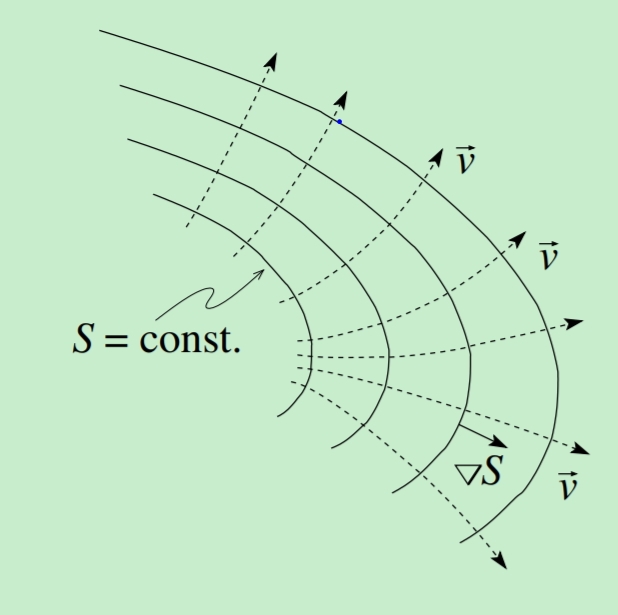
\includegraphics[scale=1]{10_1.PNG}
    \end{minipage}
    \begin{minipage}{0.5\textwidth}
        \captionsetup{font={Large}}
        \caption{The levels $S$ = const. define the wave fronts; the particles move along the gradient field $\nabla S$ with velocity $\vec{v}$.}
    \end{minipage}
\end{figure}

\textbf{One-dimensional problems:} the equations (10.12) are reduced
%公式 17
\begin{align} S^{\prime 2}-2 m(E-V) &=\hbar^{2} \frac{A^{\prime \prime}}{A} \\\left(A^{2} S^{\prime}\right)^{\prime} &=0 \end{align}
%公式 18
The latter equation can be integrated, $A$ = const./$\sqrt{S_0}$. Inserting in (10.17) gives an equation for $¨ S$ alone, but a very complex one
%公式 19
\begin{equation}
    S^{\prime 2}-2 m(E-V)=\hbar^{2}\left[\frac{3}{4}\left(\frac{S^{\prime \prime}}{S^{\prime}}\right)^{2}-\frac{1}{2}\left(\frac{S^{\prime \prime \prime}}{S^{\prime}}\right)\right]
    \end{equation}
In the WKB (Wenzel-Kramers-Brillouin) approximation we make a development of $S$ in $\hbar^2$,
%公式 20
\begin{equation}
    S=S_{0}+\hbar^{2} S_{1}+\hbar^{4} S_{2}+\cdots
    \end{equation}
Inserting in (10.19) results in\par
\textbf{0th order}
%公式 21
\begin{equation}
    S^{\prime 2} \approx S_{0}^{\prime 2}=2 m[E-V(x)]
    \end{equation}
or with the definition (10.13),
%公式 22
\begin{equation}
    S_{0}^{\prime 2}=\frac{\hbar^{2}}{\lambdabar^{2}}
    \end{equation}
which corresponds to equation (10.16), the classic limit of (10.14). The equation (10.22) can be trivially integrated for $\lambdabar<\infty$,

%公式 23
\begin{equation}
\begin{aligned} S_{0}^{\prime} &=\pm \frac{\hbar}{\lambdabar(x)}, \quad d S_{0}=\pm \frac{\hbar}{\lambdabar(x)} d x \\ S_{0}(x)-S_{0}\left(x_{0}\right) &=\pm \int_{x_{0}}^{x} d x \frac{\hbar}{\lambdabar(x)}=\pm \int_{x_{0}}^{x} d x p(x) \end{aligned}
\end{equation}
a well known result. For $¨ E> V (x)$ we get the approximate solution
%公式 24
\begin{equation}
\begin{array}{l}{\lambdabar(x) \in \mathbb{R}} \\ {\Psi(x)=\alpha \sqrt{\lambdabar(x)} \exp \left[\pm i\left(\int^{x} \frac{d x^{\prime}}{\lambdabar\left(x^{\prime}\right)}+\varphi\right)\right]}\end{array}
\end{equation}
while for $¨ E <V (x)$
%公式 25
\begin{equation}
\begin{aligned} \lbar(x) &=\frac{\hbar}{\sqrt{2 m(V(x)-E)}} \\ \Psi(x) &=\alpha \sqrt{\lbar(x)} \exp \left[\pm\left(\int^{x} \frac{d x^{\prime}}{\lbar\left(x^{\prime}\right)}+\varphi\right)\right] \end{aligned}
\end{equation}
\textbf{1st order}

%公式 26
\begin{equation}
\begin{aligned}\left(S_{0}^{\prime}+\hbar^{2} S_{1}^{\prime}\right)^{2} & \cong \underbrace{S_{0}^{\prime 2}}_{0^{\text {order }}}+\underbrace{2 \hbar^{2} S_{0}^{\prime} S_{1}^{\prime}}_{1^{\text {st }}} \\ &=\underbrace{\frac{\hbar^{2}}{\lambdabar^{2}}}_{0^\text {order }}+\underbrace{\hbar^{2} \frac{\left[\left(S_{0}^{\prime}\right)^{-1 / 2}\right]^{\prime \prime}}{\left(S_{0}^{\prime}\right)^{-1 / 2}}}_{\text 0^{order }} \\ 2 S_{0}^{\prime} S_{1}^{\prime} &=\frac{3}{4}\left(\frac{S_{0}^{\prime \prime}}{S_{0}^{\prime}}\right)^{2}-\frac{1}{2} \frac{S_{0}^{\prime \prime \prime}}{S_{0}^{\prime}} \end{aligned}
\end{equation}
We find the solution for $¨ E> V$

%公式 27
\begin{equation}
\begin{aligned} S_{0}^{\prime} &=\pm \frac{\hbar}{\lambdabar} \\ \hbar S_{1}^{\prime} &=\pm \frac{1}{2} \sqrt{\lambdabar}(\sqrt{\lambdabar})^{\prime \prime} \\ & \downarrow \operatorname{with}(\sqrt{\lambdabar})^{\prime \prime}=\frac{\lambdabar^{\prime \prime}}{2 \sqrt{\lambdabar}}-\frac{\lambdabar^{\prime 2}}{4 \lambdabar \sqrt{\lambdabar}} \\ &=\pm\left(\frac{\lambdabar^{\prime \prime}}{4}-\frac{\lambdabar^{2}}{8 \lambdabar}\right) \\ \Rightarrow \hbar S_{1} &=\pm\left(\frac{\lambdabar^{\prime}}{4}-\int^{x} d x^{\prime} \frac{\lambdabar^{\prime 2}}{8 \lambdabar}\right) \end{aligned}
\end{equation}
So that the 0th order is a good approximation,
%公式 28
\begin{equation}
    \hbar S_1\ll 1
\end{equation}
be, and with that
%公式 29
\begin{equation}
    \lambdabar'\ll 1
\end{equation}
the wavelength should only change slowly in space,

%公式 30
\begin{equation}
    \frac{\Delta\lambdabar}{\lambdabar}\ll 1
\end{equation}
with $\Delta\lambdabar=\lambdabar'\cdot\lambdabar$, the change in the wavelength over the distance $\lambdabar$, ie the relative change in $\lambdabar$.\par
A series is often put in $\hbar$ instead of $\hbar^2$: you define
%公式 13
\begin{equation}
    \Psi=e^{i W / \hbar}
    \end{equation}
with $W = S - i \hbar \operatorname{ln} A$, the development is in powers of $\hbar$,
%公式 23
\begin{equation}
    W=W_{0}+\hbar W_{1}+\hbar^{2} W_{2}+\cdots
    \end{equation}
Inserting into the complex equation (cf. (10.17))
%公式 33
\begin{equation}
    W^{\prime 2}-2 m(E-V)=i \hbar W^{\prime \prime}
    \end{equation}
%公式 34
results
%公式 35
\begin{align} W_{0}^{\prime 2} &=2 m(E-V)=\frac{\hbar^{2}}{\lambdabar^{2}} \\ 2 W_{0}^{\prime} W_{1}^{\prime} &=i W_{0}^{\prime \prime} \end{align}
with the solution
%
\begin{equation}
\begin{aligned} W_{0} &=\pm \hbar \int^{x} \frac{d x}{\lambdabar(x)} \\ W_{1} &=\frac{i}{2} \ln \frac{1}{\lambdabar(x)} \end{aligned}
\end{equation}
The 1st order correction for $\Psi$ leads to the factor
%公式 37
\begin{equation}
    \exp \left(-\frac{1}{2} \ln \frac{1}{\lambdabar}\right)=\sqrt{\lambdabar}
    \end{equation}
and is the 1st order of the WKB solution (cf. (10.24)),
%公式 38
\begin{equation}
    \Psi \sim \sqrt{\lambdabar} \exp \left[\pm i \int^{x} \frac{d x^{\prime}}{\lambdabar\left(x^{\prime}\right)}\right]
    \end{equation}
We expect a good result if $|\hbar W_1|\ll W_0$ or, since $W_0$ is monotonic if $| \hbar W_1' | \ll W_0'$. This results in the condition

%公式 39
\begin{equation}
    \frac{\lambdabar^{\prime}}{\lambdabar} \ll \frac{1}{\lambdabar} \Rightarrow \lambdabar \ll 1
    \end{equation}
in agreement with (10.29). The (classic) reversal points at which $E = V (x)$ and therefore $\lambdabar\ll\infty$ goes are obviously dangerous. At these reversal points, the wavelength changes rapidly and the WKB approximation seems to have trouble. We have to deal with these points specifically

\section{Exponential approximation}
We turn to the mathematical aspect of the WKB approximation. Given a linear differential equation of the $\text{n}^{\text{order}}$ whose leading term is multiplied by a small parameter,

%公式 40
\begin{equation}
\begin{aligned} 0=& \delta y^{(n)}+p_{n-1}(x) y^{(n-1)}+p_{n-2}(x) y^{(n-2)}+\cdots+p_{1}(x) y^{\prime}+p_{0}(x) \\ & \& \text { boundary conditions. } \end{aligned}
\end{equation}
In the limit $\delta\rightarrow 0$ the differential equation changes its order and the solution breaks down. For example, a local breakdown occurs in the following dissipative problem,
%公式 14
\begin{equation}
    \delta y^{\prime \prime}+a y^{\prime}+y=0
    \end{equation}
with $ay'$ the damping term. A global breakdown appears in the dispersive problem

%公式 42
\begin{equation}
    \delta y^{\prime \prime}+y=0
    \end{equation}
The breakdown of the solution manifests itself as follows: For $\delta\rightarrow 0$ a rapidly oscillating solution occurs, whose wavelength goes to zero with $\delta\rightarrow 0$. In the dissipative case, the oscillating solution is attenuated exponentially and the breakdown is local only; in the dispersive case, the oscillating solution is undamped and the breakdown is global.
\textbf{Simple example:}

%公式 43
\begin{equation}
\begin{aligned} \delta y^{\prime \prime}+y &=0, \quad y(0)=0, \quad y(1)=1 \\ y &=\frac{\sin (x / \sqrt{\delta})}{\sin (1 / \sqrt{\delta})}, \quad \delta \neq \frac{1}{n^{2} \pi^{2}} \end{aligned}
\end{equation}
For $\delta\rightarrow 0$ the solution oscillates strongly everywhere.\par
Dissipative and dispersive phenomena are exponential in nature [$\propto \text{exp}(x),\propto\text{exp}(ix)$] and an exponential solution is appropriate,
%公式 44
\begin{equation}
\begin{array}{c}{y(x)=A(x) \exp [S(x) / \sqrt{\delta}]} \vspace{1ex}\\ {S \text { real } \rightarrow \text { exponential behavior of the solution, }} \vspace{1ex}\\ {S \text { imaginary } \rightarrow \text { oscillating behavior of the solution. }}\end{array}
\end{equation}
The approach (10.44) combined with a development of $A$ and $S$ in $\delta$ gives the WKB approximation. In the following we restrict ourselves to problems of the type
%公式 45
\begin{equation}
    \varepsilon^{2} y^{\prime \prime}=Q(x) y
    \end{equation}
and make the approach\footnote{
    A few remarks:
    {\footnotesize{
    \begin{enumerate}
        \item[1.] In comparison with the typical problem $\hbar^2\Psi''/ 2m = [V (x) - E] \Psi$ of quantum mechanics, we note the following equivalences:
            \begin{equation}
                \begin{array}{ll}{\Psi \leftrightarrow y,} & {2 m(V-E) \leftrightarrow Q} \\ {\hbar \leftrightarrow \varepsilon,} & {\text { classic limes } \leftrightarrow \varepsilon \rightarrow 0}\end{array}
            \end{equation} 
        \item[2.] We should have a series $y\sim\operatorname{exp}[\nu^{-1}\sum\nu^nw_n]$
        begin. Then in 0th order
            \begin{equation}
                \frac{\varepsilon^{2}}{\nu^{2}} w_{0}^{\prime 2}+\cdots=Q
            \end{equation}and since $Q$ is of order $\varepsilon^0, \nu=\varepsilon$ must be.
        \item[3.] The development of (10.48) corresponds to (10.32), a development in $\hbar$.
    \end{enumerate}}}
}
%公式 46
%公式 47
%公式 48
\begin{equation}
    y(x) \sim \exp \left[\frac{1}{\varepsilon} \sum_{n=0}^{\infty} \varepsilon^{n} w_{n}(x)\right], \quad \varepsilon \rightarrow 0
    \end{equation}
Substituting (10.48) in (10.45) gives
%公式 49
\begin{equation}
    \left(w_{0}^{\prime}\right)^{2}+\varepsilon\left[2 w_{0}^{\prime} w_{1}^{\prime}+w_{0}^{\prime \prime}\right]+\varepsilon^{2}\left[2 w_{0}^{\prime} w_{2}^{\prime}+w_{1}^{\prime \prime}+\left(w_{1}^{\prime}\right)^{2}\right]+\varepsilon^{3}[\cdots]+\cdots=Q(x)
    \end{equation}
and a comparison in the different orders $\varepsilon^n$ leads to the relationships
%公式 50
\begin{equation}
\begin{aligned}\left(w_{0}^{\prime}\right)^{2} &=Q(x) \\ 2 w_{0}^{\prime} w_{1}^{\prime}+w_{0}^{\prime \prime} &=0 \\ 2 w_{0}^{\prime} w_{n}^{\prime}+w_{n-1}^{\prime \prime}+\sum_{j=1}^{n-1} w_{j}^{\prime} w_{n-j}^{\prime} &=0, \quad \text { for } n \geq 2 \end{aligned}
\end{equation}
The solutions for $w_0$ and $w_1$ are known
%公式 51
\begin{equation}
\begin{aligned} w_{0}(x) &=\pm \int^{x} d x^{\prime} \sqrt{Q\left(x^{\prime}\right)} \\ w_{1}(x) &=-\frac{1}{4} \ln Q(x) \end{aligned}
\end{equation}
where $Q$ can be real or complex. For the higher orders one finds\footnote{The orders $(\hbar=\varepsilon)^{2n}$ are integrals, the orders $(\hbar=\varepsilon)^{2n+1}$ not. This corresponds exactly to the division into $A (\hbar\;\cdot$ row in $\hbar^2$) and $S$ (row in $\hbar^2$); here we have $w$ as a series in $\hbar$.}

%公式 52
\begin{equation}
\begin{array}{ccl} w_{2} &=&\pm \int^{x} d x^{\prime}\left[\frac{Q^{\prime \prime}}{8 Q^{3 / 2}}-\frac{5\left(Q^{\prime}\right)^{2}}{32 Q^{5 / 2}}\right] \\ w_{3} &=&-\frac{Q^{\prime \prime}}{16 Q^{2}}+\frac{5\left(Q^{\prime}\right)^{2}}{6\left(Q^{\prime}\right)^{2}} \\ w_{4}&=&\pm \int^{x} d x^{\prime}\left[\frac{Q^{\prime \prime \prime \prime}}{32 Q^{5 / 2}}\right.-\frac{7 Q^{\prime} Q^{\prime \prime}}{32 Q^{7 / 2}}-\frac{19\left(Q^{\prime \prime}\right)^{2}}{128 Q^{7 / 2}} \\ &&\qquad \left.+\frac{221 Q^{\prime \prime}\left(Q^{\prime}\right)^{2}}{256 Q^{9} / 2}-\frac{1105\left(Q^{\prime}\right)^{4}}{2048 Q^{11 / 2}}\right] \\ w_{5}&=&-\frac{Q^{\prime \prime \prime} Q^{\prime \prime \prime}}{64 Q^{4}}+\frac{5\left(Q^{\prime \prime}\right)^{2}}{64 Q^{4}}-\frac{113\left(Q^{\prime}\right)^{2} Q^{\prime \prime}}{256 Q^{5}}+\frac{565\left(Q^{\prime}\right)^{4}}{2048 Q^{6}} \end{array}
\end{equation}
The first two factors are known as geometric (exp$ [w_0 / \varepsilon]$) and physical-optical ($e^{w1} = Q^{-1/4}$) approximations,
%公式 53
\begin{equation}
    \begin{aligned}
        y &\sim \exp \left[\frac{1}{\varepsilon} \sum \varepsilon^{n} w_{n}\right]\\
        &\simeq \underbrace{\exp \left[w_{0} / \varepsilon\right]}_{\text {geometric optics }} \exp \left[w_{1}\right] \exp \left[\varepsilon w_{2}\right] \cdots
    \end{aligned}
\end{equation}
The WKB series
%公式 54
\begin{equation}
    \exp \left[\frac{1}{\varepsilon} \sum_{n=0}^{\infty} \varepsilon^{n} w_{n}\right]
    \end{equation}
is an asymptotic series\footnote{
    A row
    \begin{equation}
        \sum_{n=0}^{\infty} a_{n}\left(x-x_{0}\right)^{n}
        \end{equation}
    is asymptotic to $y (x)$ for $¨ x \rightarrow x_0$ if
    \begin{equation}
        y(x)-\sum_{n=0}^{N} a_{n}\left(x-x_{0}\right)^{n} \ll\left(x-x_{0}\right)^{N+1} \quad \text { for } x \rightarrow x_{0}
        \end{equation}
    for each ¨$ N$, that is, the error (or residual term) is less than the last term considered. We then write
    \begin{equation}
        y \sim \sum_{n=0}^{\infty} a_{n}\left(x-x_{0}\right)^{n}, \quad x \rightarrow x_{0}
        \end{equation}
    where $\sim$ stands for `asymptotically the same'. For $x_0 = \infty$ is
    \begin{equation}
        y \sim \sum_{n=0}^{\infty} \frac{a_{n}}{x^{n}}, \quad x \rightarrow \infty
        \end{equation}
        an asymptotic series. The asymptotic series $\sum a_n(x-x_0)^n$ need not be convergent. The coefficients on are well defined 
        \begin{equation}
        \begin{aligned} a_{0} &=\lim _{x \rightarrow x_{0}} y(x) \\ a_{1} &=\lim _{x \rightarrow x_{0}} \frac{y(x)-a_{0}}{x-x_{0}} \\ \vdots & \vdots \\ a_{N} &=\lim _{x \rightarrow x_{0}} \frac{y(x)-\sum_{n=0}^{N-1} a_{n}\left(x-x_{0}\right)^{n}}{\left(x-x_{0}\right)^{N}} \end{aligned}
        \end{equation}
        The function $e^{-x}$ has no asymptotic development in $\infty$ since the coefficients $a_n = 0$ vanish for all $¨ n$. Thus $f$ and $f + e^{-x}$ have the same asymptotic development in $\infty$.
}, ie the solution $y$ of the differential equation (10.45) is approximated asymptotically by exp$[\sum^N \varepsilon^{n-1}w_n]$ if ​​$\varepsilon\rightarrow 0$. The WKB approximation is a singular perturbation theory in which the series in general not converged. What order do we have to go to?

We want $\sum_n\varepsilon^{n-1}w_n$ to approximate the function $y$ uniformly asymptotically in $\varepsilon$ for $\varepsilon\rightarrow 0$ over the entire interval. Then must apply
%公式 60
\begin{align} \varepsilon w_{1} & \ll w_{0}, \quad \varepsilon \rightarrow 0 \nonumber\\ \varepsilon w_{2} & \ll w_{1}, \quad \varepsilon \rightarrow 0 \nonumber\\ \vdots &\nonumber\\ \varepsilon w_{n+1} & \ll w_{n}, \quad \varepsilon \rightarrow 0 \\ \varepsilon^{N} w_{N+1} & \ll 1, \quad \varepsilon \rightarrow 0 \end{align}

%公式 16
evenly on the interval. The condition (10.61) is a consequence of the exponential approach and guarantees that the relative error is small,

%公式 62
\begin{equation}
    1-\frac{1}{y(x)} \exp \left[\sum_{n}^{N} \varepsilon^{n-1} w_{n}\right] \sim \varepsilon^{N} w_{N+1} \ll 1, \quad \varepsilon \rightarrow 0
    \end{equation}
We consider a few examples, see figure10.2.\par
%公式
$(a) \quad Q(x) = \sqrt(x)$\par
%图 2
\begin{figure}[ht]
        \centering
        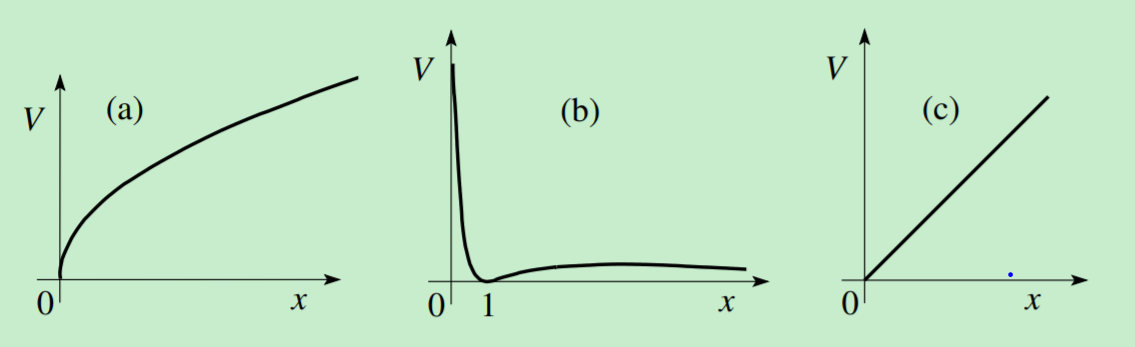
\includegraphics[scale=1]{10_2.PNG}
        \captionsetup{font={Large}}
        \caption{Potentials $Q(x)=\sqrt{x},Q(x)=[\operatorname{ln}(x)/x]^2$, and $Q (x) = x$ to the
        examples}
\end{figure}
%公式 63
\begin{equation}
    \varepsilon^{2} y^{\prime \prime}=\sqrt{x} y
    \end{equation}
Solution according to physical optics
%公式 64
\begin{equation}
\begin{aligned} w_{0} &=\pm \int d x x^{1 / 4}=\pm \frac{4}{5} x^{5 / 4} \\ w_{1} &=-\frac{1}{4} \ln \sqrt{x} \end{aligned}
\end{equation}
together this gives the solution
%公式 65
\begin{equation}
    y=c \frac{1}{\sqrt[8]{x}} \exp \left[-\frac{4}{5 \varepsilon} x^{5 / 4}\right]
    \end{equation}
The error is
%公式 66
\begin{equation}
    \left|\varepsilon w_{2}\right|=\frac{9 \varepsilon}{160} \frac{1}{x^{5 / 4}} \rightarrow 0 \quad \text { for } x \rightarrow \infty
    \end{equation}
and disappears for large values ​​of $¨ x\rightarrow\infty$.\par
%公式
%公式 67
$(b)\quad Q(x) = (\operatorname{ln}x/x)^2$
\begin{align}
    &{y^{\prime \prime}=\left(\frac{\ln x}{x}\right)^{2} y(x)} \vspace{1ex}\\ 
    &{w_{0}=\pm \int d x \frac{\ln x}{x}=\pm \frac{1}{2}(\ln x)^{2}} \vspace{1ex}\nonumber\\ 
    &{w_{1}=-\frac{1}{4} \ln \left(\frac{\ln x}{x}\right)^{2}=\frac{1}{2} \ln x-\frac{1}{2} \ln (\ln x)} \vspace{1ex}\nonumber\\ 
    &{w_{2}=\cdots=\pm\left[\frac{1}{8} \ln (\ln x) \pm \frac{3}{16} \frac{1}{(\ln x)^{2}}\right] \rightarrow \infty} \vspace{1ex}
    {\text { for } x \rightarrow \infty}\end{align}
%公式 68
Only $w_3$ is bounded for $x\rightarrow\infty$,
%公式 69
\begin{equation}
    w_{3}=\cdots=\frac{3}{16} \frac{1}{(\ln x)^{4}}-\frac{1}{16} \frac{1}{(\ln x)^{2}} \ll 1
    \end{equation}
In this case, the approximation of the physical optics is no longer sufficient.
公式
Airy functions
%公式 70
\begin{align} y^{\prime \prime} &=x y \\ w_{0} &=\pm \frac{2}{3} x^{3 / 2}\nonumber\\ w_{1} &=-\frac{1}{4} \ln x \nonumber\\ w_{2} &=\pm \frac{5}{48} \frac{1}{x^{3 / 2}} \rightarrow 0 \quad \text { für } x \rightarrow \infty \\ \Rightarrow y(x \rightarrow \infty) & \sim \frac{c}{\sqrt[4]{x}} \exp \left[\pm \frac{2}{3} x^{3 / 2}\right]\left(1 \pm \frac{5}{48} \frac{1}{x^{3 / 2}}+\cdots\right) \end{align}
%公式 17

%公式 72
\section{Reversal points}
If $Q (x)$ vanishes in $x = x_0$, i.e. $Q (x = x_0) = 0$, then $E = V (x_0)$ and we have an inversion point. The WKB approximation breaks down there
%公式 73
\begin{equation}
    w_1=-\frac{1}{4}\operatorname{ln}Q\rightarrow\infty
\end{equation}
On the other hand, the differential equation $\varepsilon^2y'' = Qy$ remains regular and the solution also exists around x0; only the WKB scheme, but not the solution, breaks down. Therefore we can continue to search for solutions to the problem. In the following we solve some typical physical problems, cf. figure 10.3, and thus come to the physical aspect of the WKB approximation.
%图 3
\begin{figure}[ht]
        \centering
        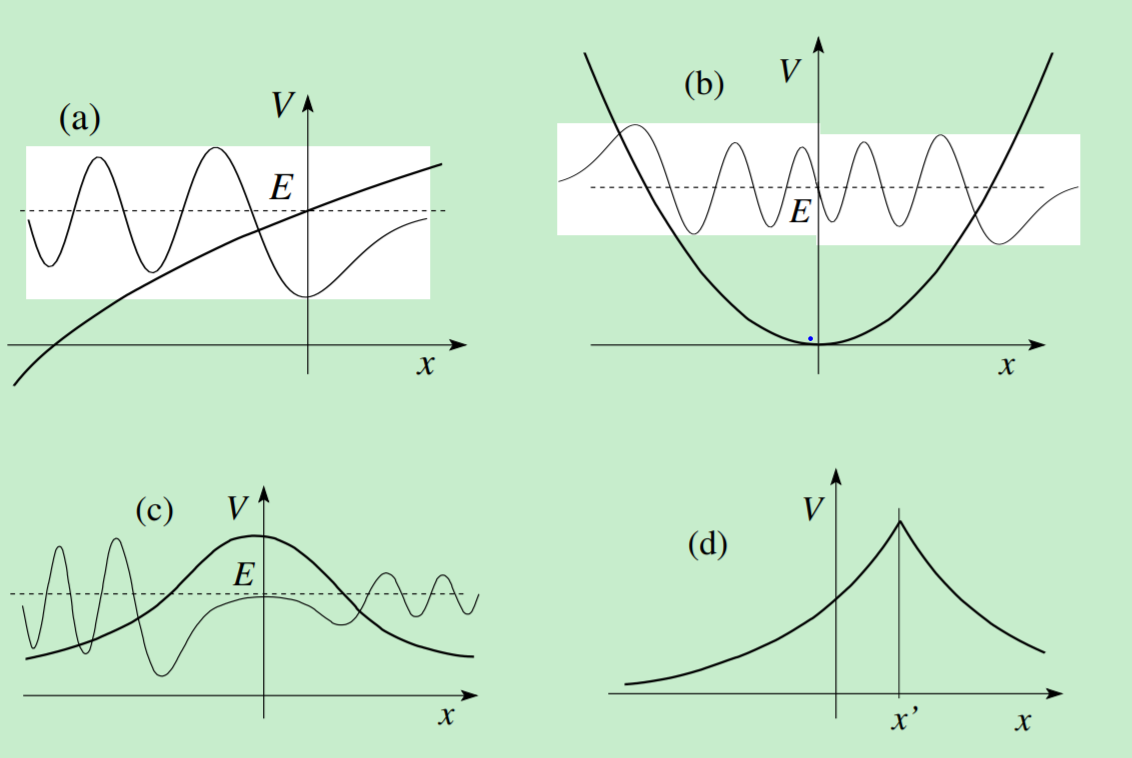
\includegraphics[scale=1]{10_3.PNG}
        \captionsetup{font={Large}}
        \caption{Sketches of some typical physical examples that are discussed below: (a) A reversal point. (b) Two reversal points that lead to an eigenvalue problem. (c) Two reversal points that lead to a tunnel problem. (d) Green's function in one dimension.}
\end{figure}
\subsection{reversal point (a)}
We start with a reversal point of the first order, cf. figure 10.4. In addition, let $| Q (x) | \gg 1 / x^2$ for $x \rightarrow\pm\infty$, for example $Q = $sinh$ x$ or $Q = x + x^3$. We divide the axis into three areas and stick the solutions in
%
\begin{figure}[ht]
    \begin{minipage}{0.5\textwidth}
        \centering
        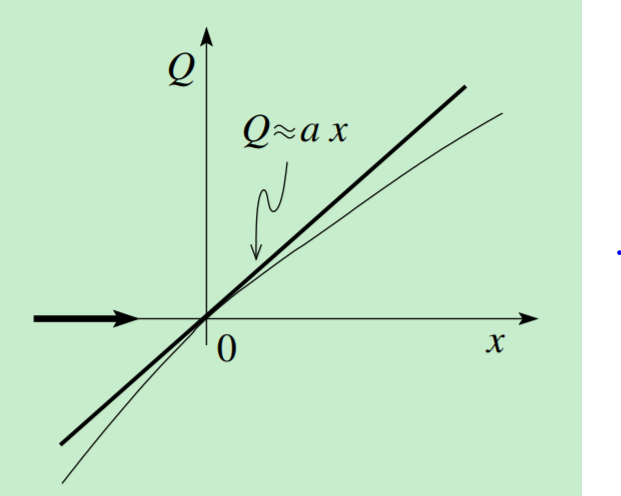
\includegraphics[scale=1]{10_4.PNG}
    \end{minipage}
    \begin{minipage}{0.5\textwidth}
        \captionsetup{font={Large}}
        \caption{Function $Q (x)$ to the turning point.}
    \end{minipage}
\end{figure}
overlapping regions as shown in figure 10.5. \par
%图 5
\begin{figure}[ht]
        \centering
        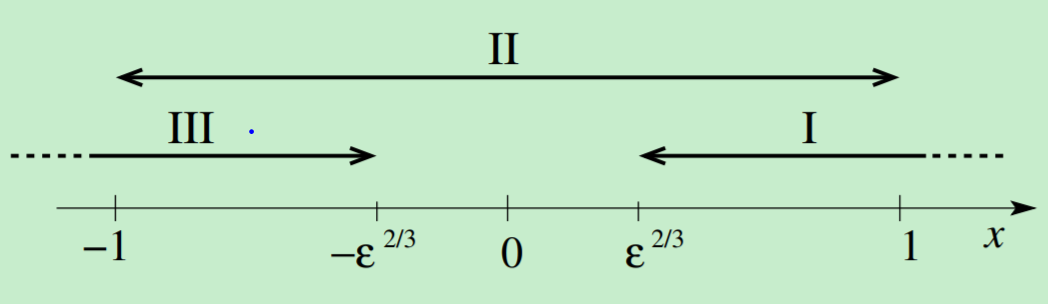
\includegraphics[scale=1]{10_5.PNG}
        \captionsetup{font={Large}}
        \caption{Overlapping regions to solve the diff equation $\varepsilon^2y''=Q(x)y$ near an inversion point.}
\end{figure}
In the regions I \& III, the WKB approximation is applicable in physical optics. There is an Airy problem in Region II.
\begin{enumerate}
    \item[I.] In area I the solution decays exponentially,
    %公式 74
    \begin{equation}
        y_{\mathrm{I}}=\frac{C}{Q^{1 / 4}} \exp \left[-\frac{1}{\varepsilon} \int_{0}^{x} d x^{\prime} \sqrt{Q\left(x^{\prime}\right)}\right]
        \end{equation}
    with $y_I (\infty) = 0$; the exponentially increasing solution exp$ [+ \int \cdots]$ does not occur. The validity of the solution requires that $w_0 / \varepsilon \gg w_1 \gg \varepsilon w_2$ and $\varepsilon w_2\ll 1$; for small $¨ x$ we ​​find the expressions with $Q \approx ax$
    %公式 75
    \begin{equation}
        \begin{array}{l}
        {w_{0} \approx \pm \frac{2 \sqrt{a}}{3} x^{3 / 2}}\vspace{1ex}\\{w_{1} \approx-\frac{1}{4} \ln x} \vspace{1ex}\\ {w_{2} \approx \pm \frac{5}{48 \sqrt{a}} x^{-3 / 2}}\end{array}
        \end{equation}
    and we get the condition $x \gg \varepsilon^{2 / 3}$
    \item[II.] We transform to the new variable
    %公式 76
    \begin{equation}
        t=\left(\frac{a}{\varepsilon^{2}}\right)^{1 / 3} x \quad \rightarrow \quad \partial_{t}^{2} y=t y
        \end{equation}
    and find the solution in the form of an Airy function,
    %公式 77
    \begin{equation}
        y_{\mathrm{II}}(x)=D \mathrm{Ai}\left[\left(\frac{a}{\varepsilon^{2}}\right)^{1 / 3} x\right]+E \mathrm{Bi}\left[\left(\frac{a}{\varepsilon^{2}}\right)^{1 / 3} x\right]
        \end{equation}
    The allowed regime is limited to $| x |\ll 1$ since the approximation $Q \approx ax$ applies only there.
    \item[III.] The solution is propagating in area III
    %公式 78
    \begin{equation}
    \begin{aligned} y_{\mathrm{III}}=& F \frac{1}{\sqrt[4]{-Q}} \exp \left[\frac{i}{\varepsilon} \int_{x}^{0} d x^{\prime} \sqrt{-Q\left(x^{\prime}\right)}\right] \\ &+G \frac{1}{\sqrt[4]{-Q}} \exp \left[-\frac{i}{\varepsilon} \int_{x}^{0} d x^{\prime} \sqrt{-Q\left(x^{\prime}\right)}\right] \end{aligned}
    \end{equation}
    The validity is limited to the area $-x\gg \varepsilon^{2 / 3}$
\end{enumerate}
The comparison of the solutions in the overlapping areas allows us to determine the coefficients $D, E, F,$ and $G$; the coefficient $C$ follows from the normalization. Area I: For small $¨ x$ we ​​write $Q \approx ax$ and get
%公式 79
\begin{equation}
    \widetilde{y_{\mathrm{I}}} \sim \frac{C}{\sqrt[4]{a x}} \exp \left[-\frac{2 \sqrt{a}}{3 \varepsilon} x^{3 / 2}\right]
    \end{equation}
Up to which $x$ can we set $Q \approx ax$? Let $Q \approx ax + bx^2$, then is
%公式 80
\begin{equation}
    w_{0} \approx \frac{2 \sqrt{a}}{3} x^{3 / 2}+\frac{b}{5 \sqrt{a}} x^{5 / 2}
    \end{equation}
and the correction generated by $b \neq 0$ is small if exp [$bx^{5 / 2} / 5\varepsilon\sqrt{a}$] $\sim 1$, i.e. $x\ll\varepsilon ^{2 / 5}$. The solution $\tilde{y}_I$ is valid in the interval $[\varepsilon^{2 / 3}, \varepsilon{2 / 5}]$ and can be compared there with $y_{II}$ (see figure 10.6),
%公式 81
\begin{equation}
    \widetilde{y_{\mathrm{I}}} \sim \frac{C}{\sqrt[4]{a x}} \exp \left[-\frac{2 \sqrt{a}}{3 \varepsilon} x^{3 / 2}\right]
    \end{equation}
can be compared to
%公式 82
\begin{equation}
    y_{\mathrm{II}} \sim \frac{1}{\sqrt{\pi}} \sqrt[6]{\frac{\varepsilon}{\sqrt{a}}} \frac{1}{\sqrt[4]{x}}\left(\frac{D}{2} \exp \left[-\frac{2 \sqrt{a}}{3 \varepsilon} x^{3 / 2}\right]+E \exp \left[\frac{2 \sqrt{a}}{3 \varepsilon} x^{3 / 2}\right]\right)
    \end{equation}
We used the asymptotics of Airyfunction for $\varepsilon\rightarrow 0$. The coefficients $D$ and $E$ result in
%公式 83
\begin{equation}
\begin{aligned} D &=\frac{2 \sqrt{\pi}}{(\varepsilon a)^{1 / 6}} C \\ E &=0 \end{aligned}
\end{equation}
We also carried out the corresponding analysis for $¨ x <0$ and compared
%$图 6
\begin{figure}[ht]
        \centering
        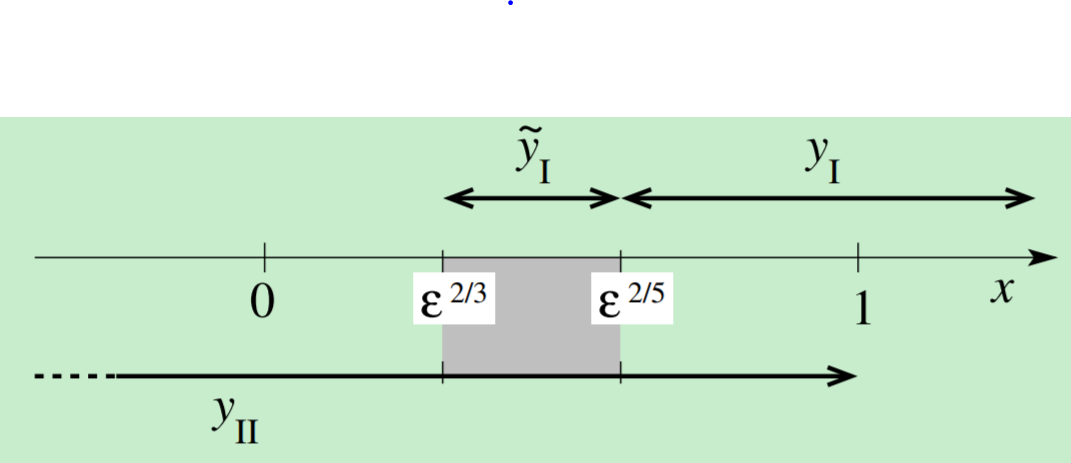
\includegraphics[scale=1]{10_6.PNG}
        \captionsetup{font={Large}}
        \caption{Overlapping regions to solve the diff equation $\varepsilon^2y''=Q(x)y$ near an inversion point. The validity areas of the printouts $y_{I},\tilde{y_I}$ and $y_{III}$ are outlined.}
\end{figure}
the Airy function (note that $E = 0$)
%公式 84
\begin{equation}
    \operatorname{Ai}(t) \sim \frac{1}{\sqrt{\pi}} \frac{1}{(-t)^{1 / 4}} \sin \left[\frac{2}{3}(-t)^{3 / 2}+\frac{\pi}{4}\right]
    \end{equation}
with the solution in area III,
%公式 85
\begin{equation}
\begin{aligned} y_{\mathrm{III}}=& \frac{F}{(-a x)^{1 / 4}} \exp \left[\frac{i 2 \sqrt{a}}{3 \varepsilon}(-x)^{3 / 2}\right] \\ &+\frac{G}{(-a x)^{1 / 4}} \exp \left[-\frac{i 2 \sqrt{a}}{3 \varepsilon}(-x)^{3 / 2}\right] \end{aligned}
\end{equation}
With $t = (a / \varepsilon^2)^{1 / 3}x$ and $D = 2\sqrt{\pi}C / (\varepsilon a)^{1/6}$ we get for $¨ y_{\text{II}}$
%公式 86
\begin{equation}
    y_{\mathrm{II}}=\frac{2 C}{(-a x)^{1 / 4}} \sin \left[\frac{2 \sqrt{a}}{3 \varepsilon}(-x)^{3 / 2}+\frac{\pi}{4}\right]
    \end{equation}
and the comparison with $y_{\text{III}}$ shows
%公式 87
\begin{equation}
    F=G^{*}=e^{i \pi / 4} C, \quad C \in \mathbb{R}
    \end{equation}
This gives us the complete solution $(\varepsilon\rightarrow 0)$
%公式 88
\begin{equation}
\begin{aligned} y_{\mathrm{I}} \;&=\;\frac{C}{Q^{1 / 4}} \exp \left[-\frac{1}{\varepsilon} \int_{0}^{x} d x^{\prime} \sqrt{Q\left(x^{\prime}\right)}\right], \quad x \geqslant \varepsilon^{2 / 3} \\ y_{\mathrm{II}} \;&\;=\frac{2 \sqrt{\pi} C}{(a \varepsilon)^{1 / 6}} \mathrm{A} \mathrm{i}\left[\left(\frac{a}{\varepsilon^{2}}\right)^{1 / 3} x\right], \quad|x| \ll 1 \\ y_{\mathrm{III}} \;&\;=\frac{2 C}{(-Q)^{1 / 4}} \sin \left[\frac{1}{\varepsilon} \int_{x}^{0} d x^{\prime} \sqrt{-Q\left(x^{\prime}\right)}+\frac{\pi}{4}\right], \quad x \ll-\varepsilon^{2 / 3} \end{aligned}
\end{equation}
\textbf{Note:} We had to start at $x\rightarrow\infty$ and derive $y_{\text{III}}$. We cannot use $y_{\text{III}}$ (as derived above) and conclude that $y_{\text{I}}$ disappears exponentially, because our analysis is only asymptotic in $\varepsilon$, that is, in leading order $\varepsilon$ correct. Specifically, be
%公式 89
\begin{equation}
    y_{\mathrm{III}}=\frac{2 C}{\sqrt[4]{-Q}} \sin \left[\frac{1}{\varepsilon} \int_{x}^{0} d x^{\prime} \sqrt{-Q}+\frac{\pi}{4}\right]
    \end{equation}
then
%公式 90
\begin{equation}
    y_{\mathrm{I}}=\frac{C}{\sqrt[4]{Q}} \exp \left[-\frac{1}{\varepsilon} \int^{x} d x^{\prime} \sqrt{Q}\right]+\mathcal{O}(\varepsilon) \exp \left[\frac{1}{\varepsilon} \int^{x} d x^{\prime} \sqrt{Q}\right]
    \end{equation}
In order to get rid of the second term in yI we need the boundary condition $y_{\text{I}} (\infty) = 0$. We therefore write the directed connection relation
\begin{equation}
    \frac{2}{\sqrt[4]{-Q}} \sin \left[\frac{1}{\varepsilon} \int_{x}^{0} d x^{\prime} \sqrt{-Q}+\frac{\pi}{4}\right] \Longleftarrow \frac{1}{\sqrt[4]{Q}} \exp \left[-\frac{1}{\varepsilon} \int_{0}^{x} d x^{\prime} \sqrt{Q}\right]
    \end{equation}
%公式 91
to continue the solution around the reversal point.\par
\textbf{Normalization:}\par
\begin{align} \int_{-\infty}^{\infty} d x y & \sim 2 C \sqrt{\frac{\pi \varepsilon}{a}} \\ \int_{-\infty}^{\infty} d x y^{2} & \sim 2 C^{2} \int_{-\infty}^{0} \frac{d x^{\prime}}{\sqrt{-Q\left(x^{\prime}\right)}} \end{align}
%公式 92
%公式 93
In (10.92) we used that only the neighborhood of 0 is relevant. The normalization factor $C$ is then chosen to suit the situation, see Bender / Orszag for further details.

\subsection{Two reversal points, eigenvalue problem (B)}
The generic eigenvalue problem with two reversal points is sketched in Figure 10.7.
%图 7
\begin{figure}[ht]
    \begin{minipage}{0.5\textwidth}
        \centering
        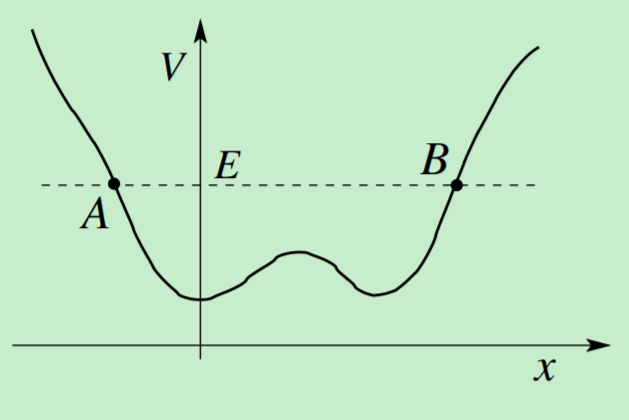
\includegraphics[scale=1]{10_7.PNG}
    \end{minipage}
    \begin{minipage}{0.5\textwidth}
        \captionsetup{font={Large}}
        \caption{Eigenvalue problem defined by the two
        Reversal points $A$ and $B$.}
    \end{minipage}
\end{figure}
We now need two connection relations (see figure 10.7): At point $A$ we need the two functions
%公式 94
\begin{equation}
    \frac{1}{\sqrt[4]{Q}} \exp \left[-\frac{1}{\varepsilon} \int_{x}^{A} d x^{\prime} \sqrt{Q}\right] \Longrightarrow \frac{2}{\sqrt[4]{-Q}} \sin \left[\frac{1}{\varepsilon} \int_{A}^{x} d x^{\prime} \sqrt{-Q}+\frac{\pi}{4}\right]
    \end{equation}
link, whereas in point B the link between the functions
%公式 95
\begin{equation}
    \frac{2}{\sqrt[4]{-Q}} \sin \left[\frac{1}{\varepsilon} \int_{x}^{B} d x^{\prime} \sqrt{-Q}+\frac{\pi}{4}\right] \Longleftarrow \frac{1}{\sqrt[4]{Q}} \exp \left[-\frac{1}{\varepsilon} \int_{B}^{x} d x^{\prime} \sqrt{Q}\right]
    \end{equation}
is to be created. In the permitted area, the two expressions ¨ $\propto$ sin [$\cdots$] must be identical (with one sign),
%公式 96
\begin{equation}
\begin{array}{l}{\sin \left[\frac{1}{\varepsilon} \int_{x}^{B} d x^{\prime} \sqrt{-Q}+\frac{\pi}{4}\right] \stackrel{!}{=} \sin \left[\frac{1}{\varepsilon} \int_{A}^{x} d x^{\prime} \sqrt{-Q}+\frac{\pi}{4}\right]} \\ {=\sin \left[\frac{1}{\varepsilon} \int_{A}^{B} d x^{\prime} \sqrt{-Q}-\left(\frac{1}{\varepsilon} \int_{A}^{x} d x^{\prime} \sqrt{-Q}+\frac{\pi}{4}\right)+\frac{\pi}{2}\right]} \\ {=-\sin \left[\frac{1}{\varepsilon} \int_{A}^{x} d x^{\prime} \sqrt{-Q}+\frac{\pi}{4}-\underbrace{\left(\frac{1}{\varepsilon} \int_{A}^{B} d x^{\prime} \sqrt{-Q}+\frac{\pi}{2}\right)}_{\Rightarrow n \pi}\right]}\end{array}
\end{equation}
This gives us the condition
%公式 97
\begin{equation}
    \frac{1}{\varepsilon} \int_{A}^{B} d x^{\prime} \sqrt{-Q}=\left(n+\frac{1}{2}\right) \pi
    \end{equation}
it defines the energy eigenvalues ​​within the framework of quantum mechanics
%公式 98
\begin{equation}
    \frac{1}{\hbar} \int_{A}^{B} d x \sqrt{2 m[E-V(x)]}=\left(n+\frac{1}{2}\right) \pi
    \end{equation}
\textbf{Generalization:} Instead of a `soft' wall with a linear potential, we can also look at hard walls. The solutions for the pot (see figure 10.8) with infinitely high walls are known,
%公式 99
\begin{equation}
\begin{aligned} \Psi & \propto \sin \frac{(n+1) \pi x}{L}, & & k=(n+1) \frac{\pi}{L} \\ \int_{0}^{L} d x k &=(n+1) \pi &=& n \pi+\frac{\pi}{2}+\frac{\pi}{2} \end{aligned}
\end{equation}
Instead of the phase shift $\pi / 4$, which we found for the linear potential, it follows from (10.99) that the shift for the hard wall is given by $\pi / 2$.(Note that the phase of the reflection coefficient $\gamma$ in 1D scattering theory is given by $\pi$. Only half the orbit (from $A$ to $B$) is considered and we get phase $\pi / 2$, just half.)
%图 8
\begin{figure}[ht]
    \begin{minipage}{0.5\textwidth}
        \centering
        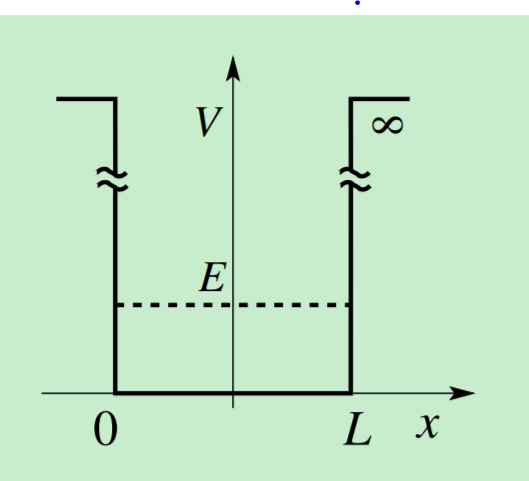
\includegraphics[scale=1]{10_8.PNG}
    \end{minipage}
    \begin{minipage}{0.5\textwidth}
        \captionsetup{font={Large}}
        \caption{The infinitely deep potential well is characterized by hard walls. The phase shifts are given by $\pi / 2$.}
    \end{minipage}
\end{figure}
In summary, we get the following quantization rule:
%公式 100
\begin{equation}
    \frac{1}{\hbar} \int_{A}^{B} d x \sqrt{2 m[E-V(x)]}=\left(n+\gamma_{A}+\gamma_{B}\right) \pi
    \end{equation}
with $\gamma_A,\gamma_B$ the phase shifts on the respective wall. The phase shifts $\gamma$ and $\gamma$ depend on the type of the reversal point, see figure 10.9. The following special cases must also be observed:\par
The special reversal point in the radial problem is only relevant for the $l = 0$ channel; for $¨ l> 0$ we have two conventional $\gamma = 1/4$ reversal points, cf. figure 10.10.\par
%图 9.10
\begin{figure}[ht]
        \centering
        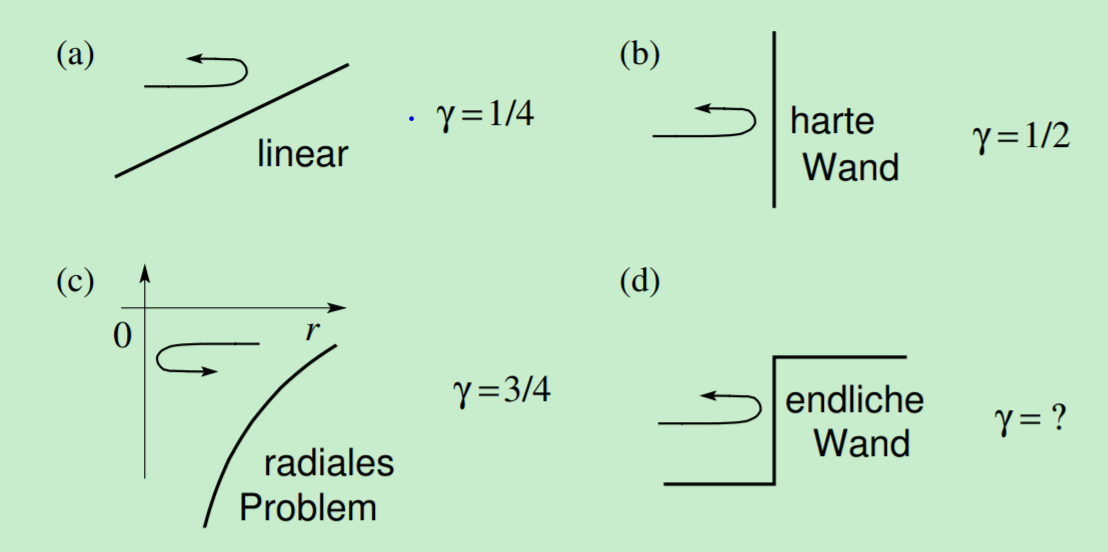
\includegraphics[scale=1]{10_9.PNG}
        \captionsetup{font={Large}}
        \caption{Different types of reversal points: (a) Linear potential with $\gamma = 1/4$. (b) Infinitely hard wall with $\gamma = 1/2$. (c) Radial problem (a 1D problem) at $r = 0$, e.g., with the attractive Coulomb potential, with $\gamma = 3/4$. (d) What value does $\gamma$ take for the finite potential level?}
\end{figure}
For $¨ l \neq 0$, the Langer rule for quasi-classical treatment must also be used
the angular momentum:
%公式 101
\begin{equation}
    l(l+1) \quad \rightarrow \quad\left(l+\frac{1}{2}\right)^{2}, \quad l \neq 0
    \end{equation}
The quantization conditions for the Coulomb problem are given by
%公式
$$
\begin{aligned} l \neq 0: & \quad\frac{1}{\hbar} \int_{r_{\min }}^{r_{\max }} d r \sqrt{2 m\left(E_{n}+\frac{Z e^{2}}{r}-\frac{(l+1 / 2)^{2} \hbar^{2}}{2 m r^{2}}\right)}=\left(n_{r}+\frac{1}{2}\right) \pi \\ &\Rightarrow E_{n}=-\frac{Z^{2} E_{R}}{n^{2}}, n=n_{r}+l+1 \end{aligned}
$$
using the effective one-dimensional potential $V_{\text{eff}}=Ze^2/r-\hbar^2(l+1/2)^2/2mr^2$.
%公式
$$
\begin{aligned} l=0: &\quad \frac{1}{\hbar} \int_{0}^{r_{\max }} d r \sqrt{2 m\left(E_{n}+\frac{Z e^{2}}{r}\right)}=\left(n_{r}+1\right) \pi=n \pi \\ & \Rightarrow E_{n}=-\frac{Z^{2} E_{R}}{n^{2}}, \quad n=n_{r}+1 \end{aligned}
$$
The quasi-classical approximation gives us the exact results for the spectrum of the hydrogen atom. However, you have to know and use a few tricks.
%图 10
\begin{figure}[ht]
        \centering
        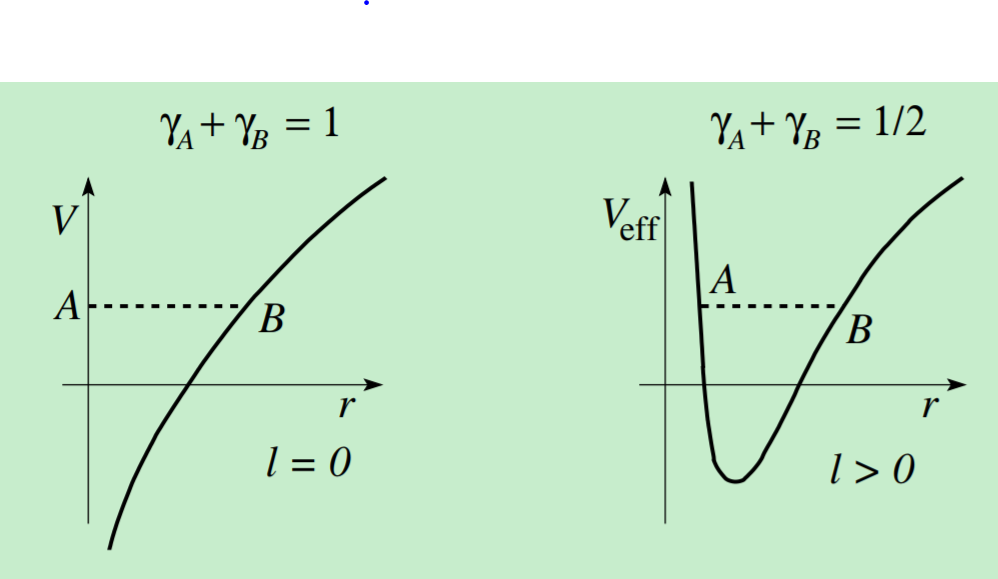
\includegraphics[scale=1]{10_10.PNG}
        \captionsetup{font={Large}}
        \caption{Phase shifts in the radial problem of the Coulomb problem for the cases $l = 0$ (left) and $l> 0$ (right). The effective potential $\text{V}_eff$ takes into account the centrifugal barrier$ \hbar^2l (l + 1) / 2mr^2$.}
\end{figure}
\subsection{Tunnel problems (C)}
The tunnel problem involves a potential with a classically forbidden zone as outlined in figure 10.11. The boundary conditions correspond to
\begin{figure}[ht]
    \begin{minipage}{0.5\textwidth}
        \centering
        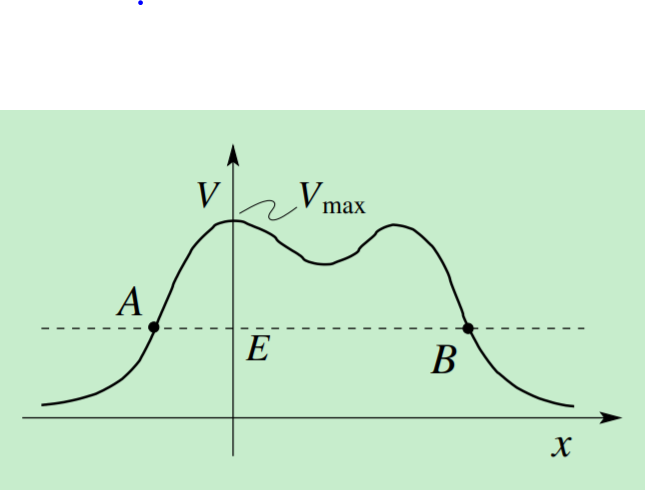
\includegraphics[scale=1]{10_11.PNG}
    \end{minipage}
    \begin{minipage}{0.5\textwidth}
        \captionsetup{font={Large}}
        \caption{Tunnel problem defined by two reversal points $A$ and $B$. We require that the potential at ± $\pm\infty$ disappears quickly enough, $V(x\rightarrow\infty)\rightarrow 0$ faster than $1 / x$}
    \end{minipage}
\end{figure}
that of a scattering process, with an incident and a reflected wave for $x\rightarrow-\infty$, and a transmitted wave for $x\rightarrow\infty$,
%公式 102
\begin{equation}
\begin{array}{l}{y(x) \sim e^{i k x}+r e^{-i k x}, \quad \text { for } x \rightarrow-\infty} \\ {y(x) \sim t e^{i k x}, \quad \text { for } x \rightarrow \infty}\end{array}
\end{equation}
The wave vector k defines the particle energy $E = \hbar^2k^2 / 2m$. We need the differential equation
%
\begin{equation}
    \varepsilon^{2} y^{\prime \prime}=Q(x) y
    \end{equation}
solve and take into account a new type of reversal points, cf. figure 10.12 corresponding to point B in figure 10.11.
%图 12
\begin{figure}[ht]
    \begin{minipage}{0.5\textwidth}
        \centering
        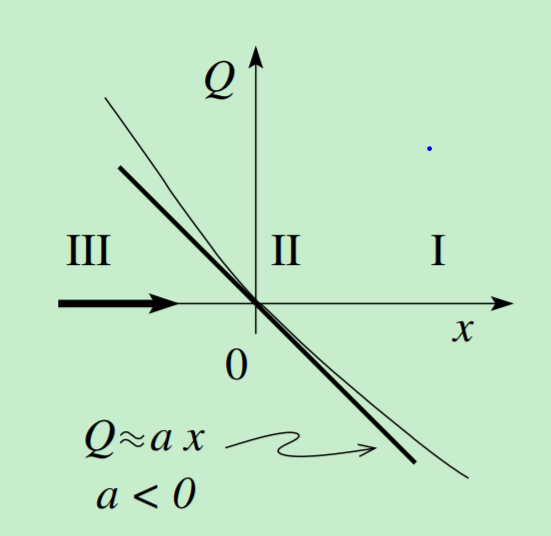
\includegraphics[scale=1]{10_12.PNG}
    \end{minipage}
    \begin{minipage}{0.5\textwidth}
        \captionsetup{font={Large}}
        \caption{Reversal point to exit the forbidden zone at B.}
    \end{minipage}
\end{figure}
We start with region I and work on region II to III. The propagating solution in region I,
%公式 104
\begin{equation}
    y_{\mathrm{I}}(x)=\frac{1}{\sqrt[4]{-Q}} \exp \left[\frac{i}{\varepsilon} \int_{0}^{x} d x^{\prime} \sqrt{-Q}\right]
    \end{equation}
$x> 0$, we can write near 0 using the expansion $Q (x) \approx ax$, $a <0$ as
%公式 105
\begin{equation}
    y_{\mathrm{I}} \sim \frac{1}{(-a x)^{1 / 4}} \exp \left[\frac{2 i \sqrt{-a}}{3 \varepsilon} x^{3 / 2}\right], \quad x \rightarrow 0
    \end{equation}
On the other hand, with $t = (−a / \varepsilon^2)^{1 / 3}x, y'' = −ty$ and in region II around $x = 0$ we find the solution
%公式 106
\begin{equation}
\begin{aligned} y_{\mathrm{II}}(x)=& \alpha \mathrm{Ai}\left[-\left(\frac{-a}{\varepsilon^{2}}\right)^{1 / 3} x\right]+\beta \mathrm{Bi}\left[-\left(\frac{-a}{\varepsilon^{2}}\right)^{1 / 3} x\right] \\ \sim & \frac{1}{\sqrt{\pi}}\left(\frac{\varepsilon}{\sqrt{-a}}\right)^{1 / 6} \frac{1}{\sqrt[4]{x}}\left[\alpha \sin \left(\frac{2 \sqrt{-a}}{3 \varepsilon} x^{3 / 2}+\frac{\pi}{4}\right)\right.\\ &\left.+\beta \cos \left(\frac{2 \sqrt{-a}}{3 \varepsilon} x^{3 / 2}+\frac{\pi}{4}\right)\right] \end{aligned}
\end{equation}
A comparison of the solutions in areas I and II, (10.105) and (10.106) provides the relationships
%公式 107
\begin{equation}
\begin{aligned} \alpha &=\frac{\sqrt{\pi}}{(-\varepsilon a)^{1 / 6}} e^{i \pi / 4} \\ \beta &=\frac{\sqrt{\pi}}{(-\varepsilon a)^{1 / 6}} e^{-i \pi / 4} \end{aligned}
\end{equation}
In region III, Ai decays exponentially and only the solution
%公式
$$
    \mathrm{Bi}\left[-\left(\frac{-a}{\varepsilon^{2}}\right)^{1 / 3} x\right] \sim \frac{1}{\sqrt{\pi}}\left(\frac{\varepsilon}{\sqrt{-a}}\right)^{1 / 6} \frac{1}{(-x)^{1 / 4}} \exp \left[\frac{2 \sqrt{-a}}{3 \varepsilon}(-x)^{2 / 3}\right]
$$
survives asymptotically for $x\rightarrow-\infty$ (Ai is subdominant for $x\rightarrow-\infty$). So is
%公式 108
\begin{equation}
\begin{aligned} y_{\mathrm{III}}(x) &=\underbrace{\frac{\sqrt{\pi}}{(-\varepsilon a)^{1 / 6}} e^{-i \pi / 4}}_{\beta} \frac{1}{\sqrt{\pi}}\left(\frac{\varepsilon}{\sqrt{-a}}\right)^{1 / 6} \frac{1}{(-x)^{1 / 4}} \exp \left[\frac{2 \sqrt{-a}}{3 \varepsilon}(-x)^{2 / 3}\right] \\ &=\frac{1}{Q^{1 / 4}} \exp \left[\frac{1}{\varepsilon} \int_{x}^{0} d x^{\prime} \sqrt{Q}-\frac{i \pi}{4}\right] \end{aligned}
\end{equation}
We get the following connection rules (cf. (10.91) and figure 10.13), at $A$
%公式 109
\begin{equation}
    \frac{1}{\sqrt[4]{-Q}} \exp \left[\frac{i}{\varepsilon} \int_{x}^{A} d x^{\prime} \sqrt{-Q}\right] \Longrightarrow \frac{1}{\sqrt[4]{Q}} \exp \left[\frac{1}{\varepsilon} \int_{A}^{x} d x^{\prime} \sqrt{Q}-\frac{i \pi}{4}\right]
    \end{equation}
and at $B$,
%gs 110
\begin{equation}
    \frac{1}{\sqrt[4]{Q}} \exp \left[\frac{1}{\varepsilon} \int_{x}^{B} d x^{\prime} \sqrt{Q}-\frac{i \pi}{4}\right] \Longleftarrow \frac{1}{\sqrt[4]{-Q}} \exp \left[\frac{i}{\varepsilon} \int_{B}^{x} d x^{\prime} \sqrt{-Q}\right]
    \end{equation}
%图 13
\begin{figure}[ht]
    \begin{minipage}{0.5\textwidth}
        \centering
        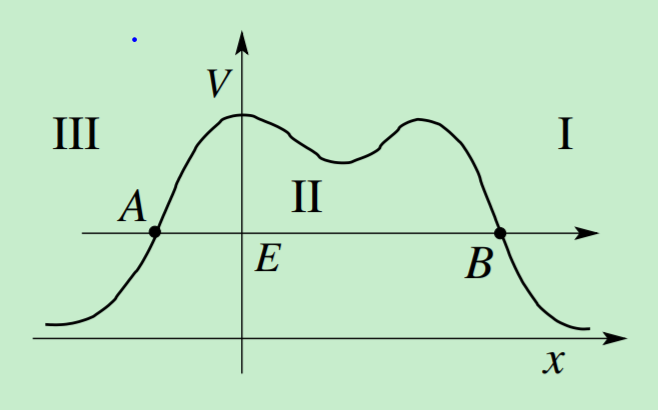
\includegraphics[scale=1]{10_13.PNG}
    \end{minipage}
    \begin{minipage}{0.5\textwidth}
        \captionsetup{font={Large}}
        \caption{Connection rules to the tunnel problem.}
    \end{minipage}
\end{figure}
Back to the tunnel problem: we define
%gs 111
\begin{equation}
\begin{aligned} k(x) & \equiv \frac{1}{\hbar} \sqrt{2 m[E-V(x)]}, \quad x<A \quad \& \quad B<x \\ \kappa(x) & \equiv \frac{1}{\hbar} \sqrt{2 m[V(x)-E]}, \quad A<x<B \end{aligned}
\end{equation}
We continue to write
%公式 112
\begin{equation}
    \int_{B}^{x} d x^{\prime} k\left(x^{\prime}\right) \quad \rightarrow \quad k x+I \quad \text { for } x \rightarrow \infty
    \end{equation}
With
%公式 113
\begin{equation}
    I=\int_{B}^{\infty} d x^{\prime}\left[k\left(x^{\prime}\right)-k\right]-B k, \quad k=\sqrt{2 m E} / \hbar
    \end{equation}
The transmitted wave for $x\rightarrow\infty$ should have the form $ y_{\text{I}}\sim t\,\text{exp} [ikx]$ asymptotically and accordingly we apply the following expression,
\begin{equation}
    y_{\mathrm{I}}=t \sqrt{\frac{k}{k(x)}} \exp [-i I] \exp \left[i \int_{B}^{x} d x^{\prime} k\left(x^{\prime}\right)\right]
    \end{equation}
%公式 114
The continuation into area II gives, see (10.110),
%公式 115
\begin{equation}
\begin{aligned} y_{\mathrm{II}} &\;=t \sqrt{\frac{k}{\kappa(x)}} \exp [-i I] \exp \left[-\frac{i \pi}{4}\right] \exp \left[\int_{x}^{B} d x^{\prime} \kappa\left(x^{\prime}\right)\right] \\ \;&\;=t \sqrt{\frac{k}{\kappa(x)}} \exp [-i I] \exp \left[-\frac{i \pi}{4}\right] \\ & \qquad \cdot \exp \left[\int_{A}^{B} d x^{\prime} \kappa\left(x^{\prime}\right)\right] \underbrace{\exp }\left[-\int_{A}^{x} d x^{\prime} \kappa\left(x^{\prime}\right)\right]
\end{aligned}
\end{equation}
The factor ∗ describes the exponential decay of the wave function in the forbidden region $x> A$. Finally we continue the solution with the help of (10.91) into region III with $x <A,$
%公式 116
\begin{equation}
\begin{aligned} y_{\mathrm{III}}=& 2 t \sqrt{\frac{k}{k(x)}} \exp [-i I] \exp \left[-\frac{i \pi}{4}\right] \\ & \times \exp \left[\int_{A}^{B} d x^{\prime} \kappa\left(x^{\prime}\right)\right] \sin \left[\int_{x}^{A} d x^{\prime} k\left(x^{\prime}\right)+\frac{\pi}{4}\right] \end{aligned}
\end{equation}
We define
%公式 117
\begin{equation}
\begin{aligned} \int_{x}^{A} k\left(x^{\prime}\right) d x^{\prime} & \sim-x k+J, \text { mit } \\ J &=A k+\int_{-\infty}^{A} d x^{\prime}\left[k\left(x^{\prime}\right)-k\right] \end{aligned}
\end{equation}
and find the expression
%公式 118
\begin{equation}
\begin{aligned} y_{\mathrm{III}} &=t \sqrt{\frac{k}{k(x)}} \exp [-i I] \exp \left[\int_{A}^{B} d x^{\prime} \kappa\left(x^{\prime}\right)\right] \exp \left[-\frac{3 \pi i}{4}\right] \\ & \times\left(\exp \left[i \int_{x}^{A} d x^{\prime} k\left(x^{\prime}\right)+\frac{i \pi}{4}\right]+\exp \left[-i \int_{x}^{A} d x^{\prime} k\left(x^{\prime}\right)-\frac{i \pi}{4}\right]\right) \\ & \quad \quad \quad \quad \text { für } x \rightarrow-\infty \\ & \sim t \exp [-i I] \exp \left[\int_{A}^{B} d x^{\prime} \kappa\left(x^{\prime}\right)\right]\left(\frac{1}{i} e^{-i k x-i J}-e^{i k x-i J}\right) \\ & \sim t \exp \left[\int_{A}^{B} d x^{\prime} \kappa\left(x^{\prime}\right)\right]\left(-i e^{i(J-I)} e^{-i k x}-e^{-i(J+I)} e^{i k x}\right) \end{aligned}
\end{equation}
The comparison with (10.102) provides
%公式 119
\begin{equation}
\begin{aligned}-& t \exp \left[\int_{A}^{B} d x^{\prime} \kappa\left(x^{\prime}\right)\right] \exp [-i(J+I)]=& 1 \\-& i t \exp \left[\int_{A}^{B} d x^{\prime} \kappa\left(x^{\prime}\right)\right] \exp [i(J-I)]=r \end{aligned}
\end{equation}
This determines the transmission amplitude and probability
%公式 102
\begin{equation}
\begin{array}{rl}
\text { T-Amplitude: } & \quad t=-\exp [i(I+J)] \exp \left[-\int_{A}^{B} d x^{\prime} \kappa\left(x^{\prime}\right)\right] \\ 
\text { T-Probability: } &\quad|t|^{2}=\exp \left[-2 \int_{A}^{B} d x^{\prime} \kappa\left(x^{\prime}\right)\right]
\end{array}
\end{equation}
The reflection parameters result in
%公式 112
\begin{eqnarray} 
    \text { R-Amplitude: } & r&=i e^{2 i J}\nonumber\\ 
    \text { R-Probability: } &|r|^{2} &\sim 1 \\ 
    \text { more accurate: } & &\sim 1-|t|^{2} 
\end{eqnarray}
%公式 122
(10.121) only takes into account the leading order.
\subsection{Green functions (D)}
We search the Green’s function for the one-dimensional problem defined by
%公式 123
\begin{equation}
    \left[\varepsilon^{2} \partial_{x}^{2}-Q(x)\right] G\left(x, x^{\prime}\right)=\delta\left(x-x^{\prime}\right), \quad G\left(\pm \infty, x^{\prime}\right)=0
    \end{equation}
%图 14
\begin{figure}[ht]
    \begin{minipage}{0.6\textwidth}
        \centering
        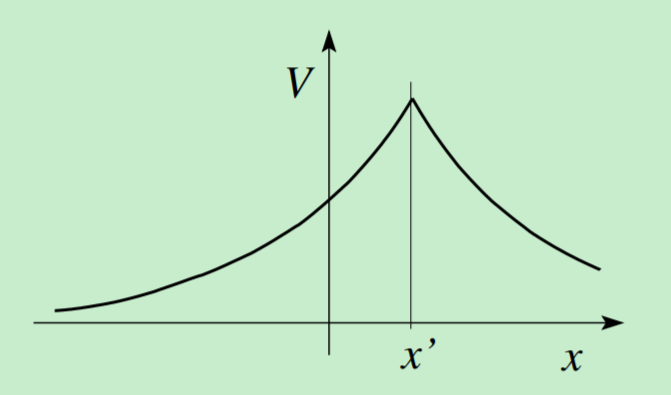
\includegraphics[scale=1]{10_14.PNG}
    \end{minipage}
    \begin{minipage}{0.4\textwidth}
        \captionsetup{font={Large}}
        \caption{Green's function $G(x,x')$}
    \end{minipage}
\end{figure}
We apply a WKB solution for $¨ x> x_0$ and for $¨ x <x_0$ and use the exponentially vanishing solutions. Then the solutions are put together in such a way that $\partial_xG> - \partial_xG \leq 1 / \varepsilon^2$, cf. figure 10.14. The result is in the form 
\begin{equation}
    G\left(x, x^{\prime}\right)=-\frac{1}{2 \varepsilon} \frac{1}{\sqrt[4]{Q(x) Q\left(x^{\prime}\right)}} \exp \left[-\frac{1}{\varepsilon}\left|\int_{x^{\prime}}^{x} d y \sqrt{Q(y)}\right|\right] 
    \end{equation}
%公式 124